\chapter{Metodologia e Desenvolvimento}

Este capítulo detalha o percurso metodológico adotado, as decisões arquiteturais e a validação
do MVP de anamnese assistida.

\section{Classificação da Pesquisa}

\subsection{Quanto à Natureza}

A pesquisa é aplicada, pois busca resolver problema prático de estruturação de dados clínicos
em anamnese.

\subsection{Quanto aos Objetivos}

Trata-se de pesquisa exploratória, com levantamento bibliográfico e avaliação de viabilidade
técnica da integração entre LLM e NER.

\subsection{Quanto aos Procedimentos Técnicos}

Adotou-se abordagem experimental e prototipagem, com implementação de MVP para validação
da hipótese arquitetural.

\section{Requisitos do Sistema}

\subsection{Requisitos Funcionais}

\begin{itemize}
\item RF01: Interação em linguagem natural por chat.
\item RF02: Condução de anamnese com uma pergunta por vez.
\item RF03: Extração automática de entidades clínicas.
\item RF04: Gestão de contexto da conversa por sessão.
\item RF05: Sanitização de artefatos técnicos nas respostas.
\end{itemize}

\subsection{Requisitos Não Funcionais}

\begin{itemize}
\item RNF01: Latência de inferência até 5 segundos.
\item RNF02: Não exposição de chaves de API no cliente.
\item RNF03: Interoperabilidade com saída em JSON.
\item RNF04: Tolerância a falhas temporárias de inferência externa.
\end{itemize}

\section{Arquitetura da Solução}

A solução foi arquitetada com padrão Backend for Frontend (BFF), no qual o servidor Node.js
orquestra chamadas entre frontend e serviços de IA.

\begin{figure}[htb]
  \centering
  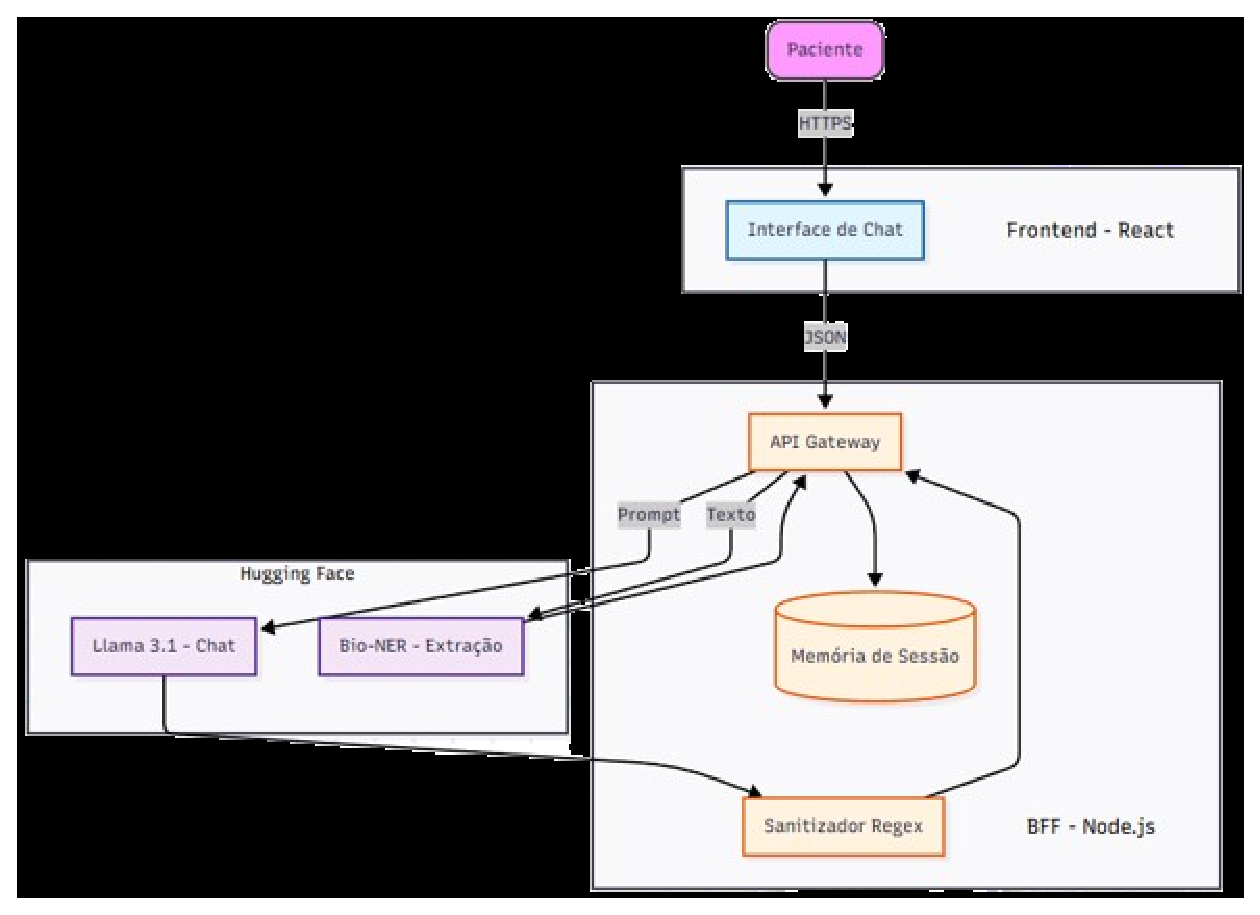
\includegraphics[width=0.90\textwidth]{figuras/arquitetura-solucao.eps}
  \caption{Diagrama de fluxo de dados e componentes da arquitetura proposta.}
  \label{fig:arquitetura-solucao}
\end{figure}

\section{Modelagem do Sistema}

\subsection{Diagrama de Sequência}

\begin{figure}[htb]
  \centering
  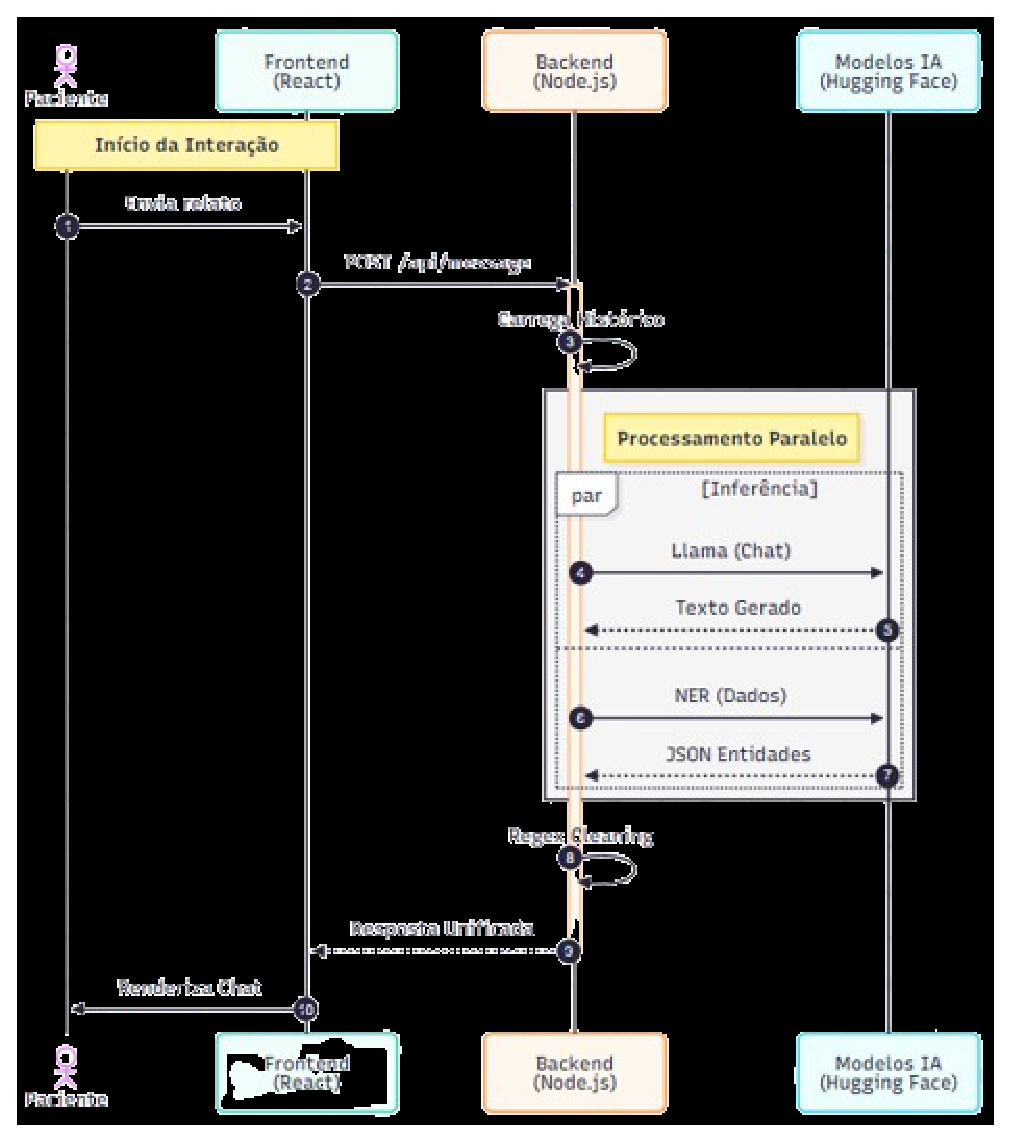
\includegraphics[width=0.90\textwidth]{figuras/sequencia.eps}
  \caption{Diagrama de sequência do fluxo de mensagem.}
  \label{fig:sequencia}
\end{figure}

\subsection{Diagrama de Componentes}

\begin{figure}[htb]
  \centering
  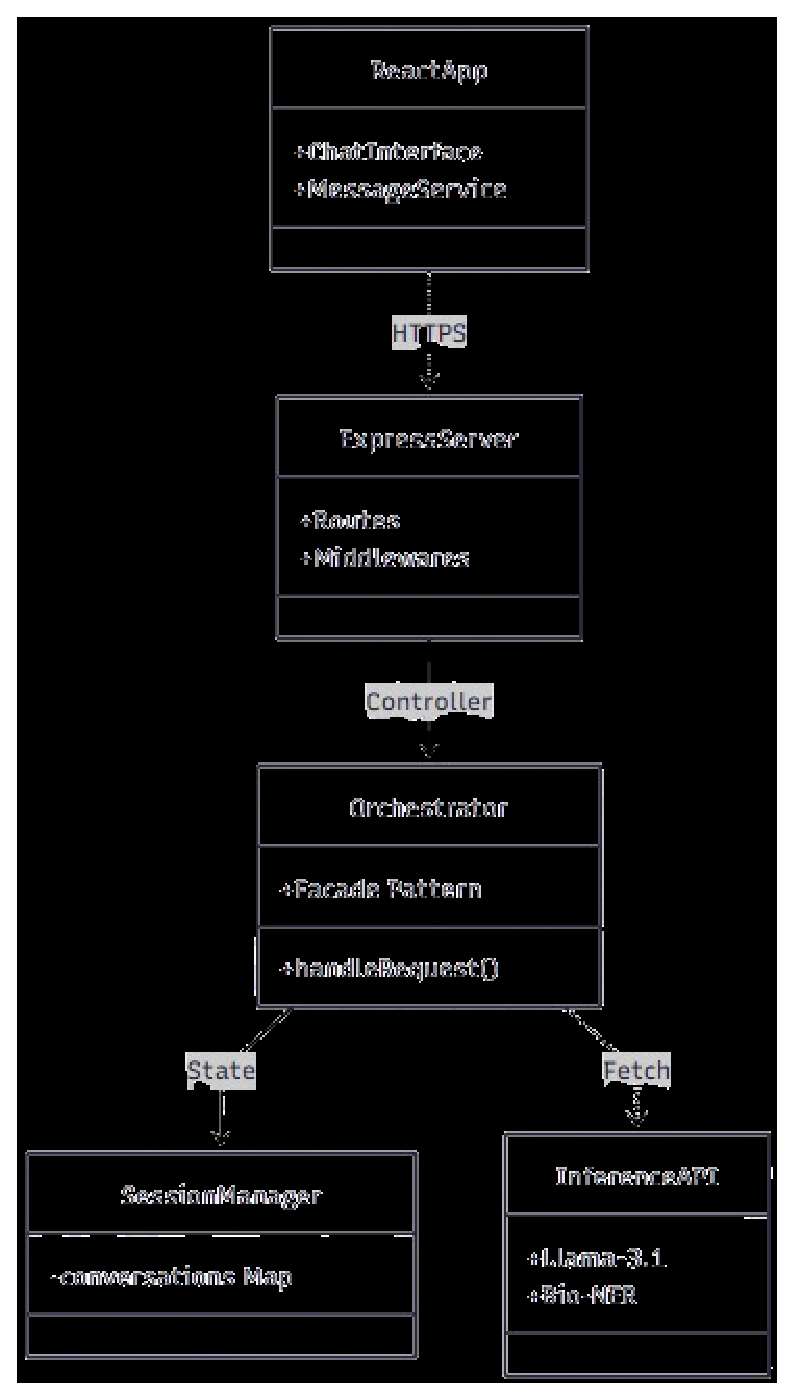
\includegraphics[width=0.90\textwidth]{figuras/componentes.eps}
  \caption{Diagrama de componentes da arquitetura BFF.}
  \label{fig:componentes}
\end{figure}

\section{Tecnologias e Ferramentas}

Foi adotada uma pilha JavaScript/TypeScript com React no frontend, Node.js e Express no
backend, Vite como ferramenta de desenvolvimento e a Hugging Face Inference API para
consumo dos modelos.

\section{Estratégia de Inteligência Artificial Híbrida}

O componente generativo usa \texttt{meta-llama/Llama-3.1-8B-Instruct} para condução do
diálogo clínico. O componente extrativo usa \texttt{d4data/biomedical-ner-all} para
classificação de entidades.

\section{Gestão de Estado e Sanitização}

O estado de sessão é mantido em memória por \texttt{userId}, garantindo continuidade da
anamnese. A sanitização aplica limpeza de artefatos de metadados com padrões de regex antes
do retorno ao cliente.

\section{Planejamento de Testes e Validação}

Foram definidos casos de teste para sintomas únicos, negações, múltiplos sintomas e presença de
medicação, com critérios de aceitação voltados à qualidade da pergunta do chat e precisão de
entidades extraídas.

\section{Resultados Preliminares do MVP}

\subsection{Análise Qualitativa da Interação}

Após ajuste de temperatura para 0.4 e refinamento de prompt, o modelo apresentou boa aderência
à persona clínica, com redução de respostas fora de contexto.

\subsection{Desempenho da Extração de Entidades}

O modelo NER identificou com boa precisão sintomas e medicamentos frequentes. A principal
limitação observada foi desambiguação de negações complexas, indicando necessidade de módulo
de detecção de negação no TCC 2.

\subsection{Métricas de Latência}

O tempo de resposta fim a fim oscilou entre 2.5 e 4.0 segundos, aceitável para MVP acadêmico,
mas com espaço para otimização por streaming e melhorias de infraestrutura.

\section{Interface do Usuário e Validação do MVP}

\begin{figure}[htb]
  \centering
  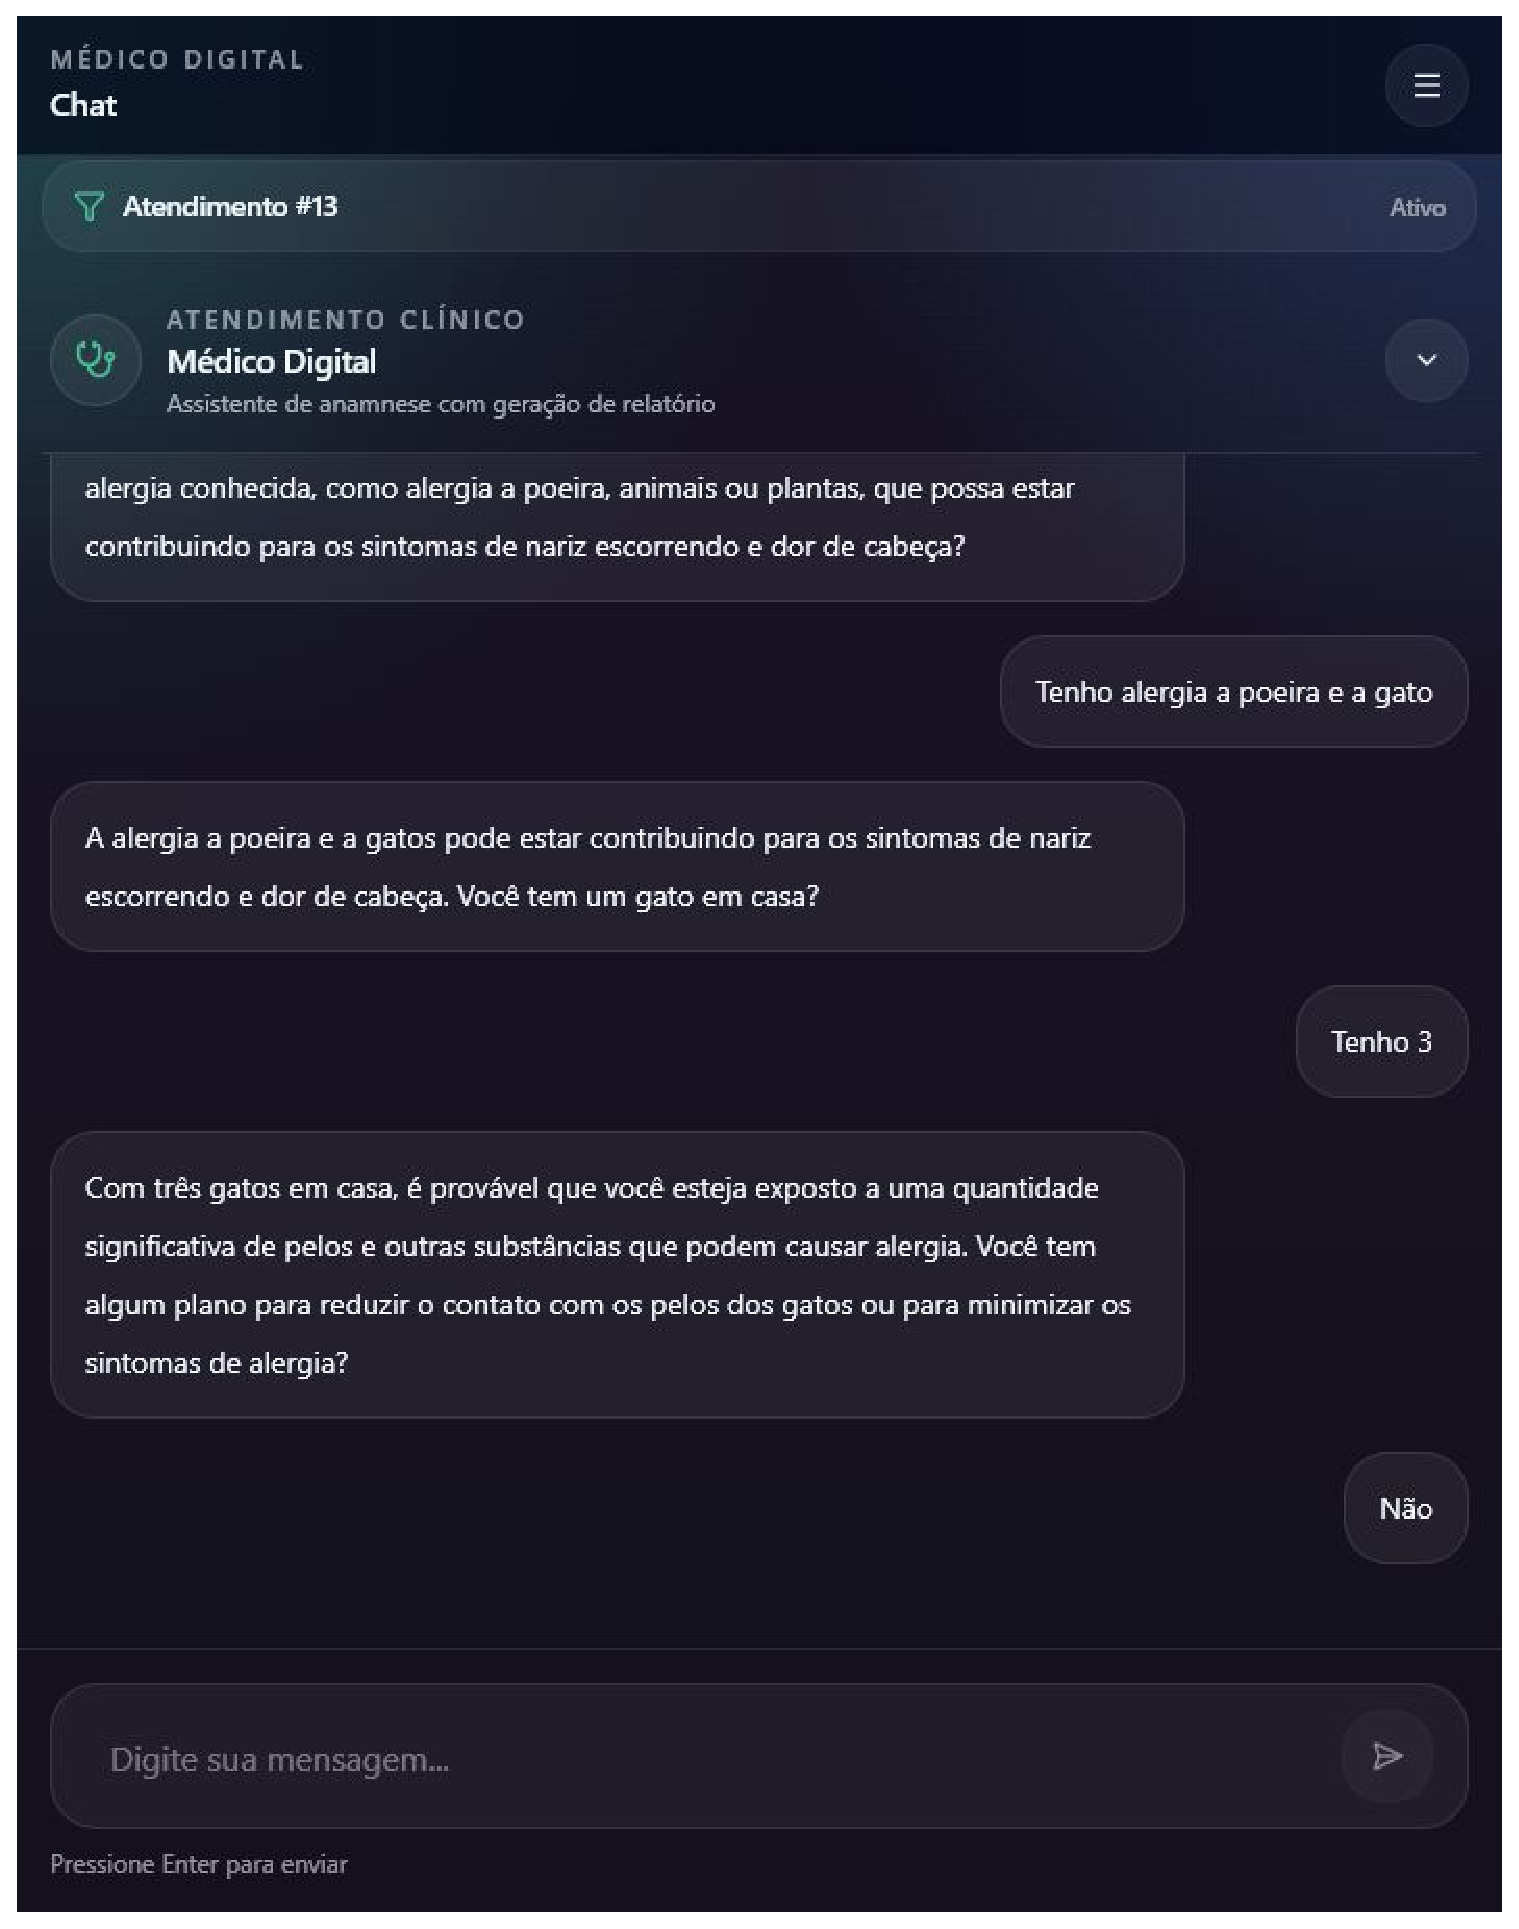
\includegraphics[width=0.85\textwidth]{figuras/print-chat.eps}
  \caption{Interface de interação do paciente com o chatbot médico.}
  \label{fig:print-chat}
\end{figure}

A interface React priorizou clareza visual, feedback de carregamento e manutenção de contexto
conversacional.

\chapter{Considerações Finais e Cronograma}

O TCC 1 atingiu o objetivo de validar uma arquitetura híbrida para anamnese assistida. A
abordagem com BFF, modelo generativo e componente extrativo mostrou viabilidade técnica e
potencial para evolução em ambiente real.

\section{Limitações Atuais e Trabalhos Futuros}

\begin{itemize}
\item Implementação de RAG para reduzir alucinações e fundamentar respostas em base curada.
\item Persistência em banco relacional e autenticação para continuidade longitudinal do cuidado.
\item Expansão da plataforma web além do chat, com requisitos de responsividade e acessibilidade.
\item Validação com usuários reais para refinamento da persona e da comunicação clínica.
\end{itemize}

\section{Cronograma de Atividades (TCC 2)}

\begin{table}[htb]
\centering
\caption{Cronograma de atividades previstas para o TCC 2 (4 meses).}
\label{tab:cronograma-tcc2}
\begin{tabular}{lcccc}
\hline
Atividade / Mês & Mês 1 & Mês 2 & Mês 3 & Mês 4 \\
\hline
Infraestrutura de Dados e Segurança & X &   &   &   \\
Implementação do RAG e Vetorização  & X & X &   &   \\
Consolidação da Plataforma Web      &   & X & X &   \\
Testes de Usabilidade e Refinamento &   &   & X &   \\
Escrita da Monografia Final e Defesa&   &   & X & X \\
\hline
\end{tabular}
\end{table}

O TCC 2 concentra dois desafios centrais: o desafio algorítmico de integração de RAG com
garantia de segurança clínica e o desafio de engenharia full stack para consolidar o fluxo
completo da aplicação com alta usabilidade.
\part{Texto e Pós Texto}
